% !TEX output_directory=output
%%%%%%%%%%%%%%%%%%%%%%%%%%%%%%%%%%%%%%%%%%%%%%%%%%%%%%%%%%%%%%%%%%%%%%%%%%%%
% !TEX root = main.tex
\documentclass[a4paper,10pt]{article}
\pdfinfo{
     /Title Internationaler Vergleich der Digitalisierung der Krankenhauslandschaft
     /Subject Hauptseminar
     /Author Johannes Wolf
}
\title{Internationaler Vergleich der Digitalisierung der Krankenhauslandschaft:
Treibergrößen und Defizitbereiche in Deutschland}
\author{Johannes Wolf}
\date{\today}

%%%%%%%%%%%%%%%%%%%%%%%%%%%%%%%%%%%%%%%%%%%%%%%%%%%%%%%%%%%%%%%%%%%%%%%%%%%%
% Includes
%%%%%%%%%%%%%%%%%%%%%%%%%%%%%%%%%%%%%%%%%%%%%%%%%%%%%%%%%%%%%%%%%%%%%%%%%%%%
\usepackage[utf8]{inputenc}
\usepackage{csquotes}
\usepackage[german]{babel}
\usepackage[T1]{fontenc}
\usepackage[margin=23mm,bottom=30mm]{geometry}
\usepackage[table,usenames,dvipsnames]{xcolor}
\usepackage{graphicx, wrapfig, helvet, titlesec, fancyhdr}
\usepackage[germankw,german]{algorithm2e}
\usepackage{tikz}
\usepackage{tikz-qtree}
\usepackage{eurosym}
\usetikzlibrary{trees}
\tikzset{
  treenode/.style = {shape=rectangle, rounded corners,
                     draw, align=center},
  root/.style     = {treenode, font=\Large, bottom color=red!30},
  env/.style      = {treenode, font=\ttfamily\normalsize},
  dummy/.style    = {circle,draw}
}
\usepackage{amsmath,amsfonts,amssymb,amsthm}
\usepackage{hyperref} % verwandelt alle Kapitelüberschriften, Verweise aufs Literaturverzeichnis und andere Querverweise in PDF-Hyperlinks
\hypersetup{
	pdftitle={Internationaler Vergleich der Digitalisierung der Krankenhauslandschaft},
	pdfauthor={Johannes Wolf},
	pdfborder={0 0 0} % entfernt hässliche Kästen um Links
}
\usepackage[%
  backend=biber      % biber or bibtex
 ,style=authortitle
 ,citestyle=authoryear-comp %authoryear-icomp
 % ,sorting=none        % no sorting
 ,sorting=nyt         % name, year, title
 ,dashed=false        % so author names aren't replaced by a dash
 ,block=none
 ,indexing=false
 ,citereset=none
 ,isbn=true
 ,url=true
 ,doi=true            % prints doi (digital object identifier)
 ,natbib=true         % if you need natbib functions
 ,language=german
 ,maxcitenames=1			% Cite as 'Name et al.' if there are multiple authors
]{biblatex}
\addbibresource{Quellen.bib}  % better than \bibliography
\DefineBibliographyStrings{german}{
	bibliography = {Literaturverzeichnis},
  andothers = {et al.}
}
\defbibheading{bibliography}[\bibname]{%
	 \noindent\LARGE\textbf{\textcolor{thmgrey}#1}
}

% define color used for titels. Offical color of the thm
\definecolor{thmgrey}{HTML}{4a5c66}
\definecolor{green}{HTML}{4E9A06}

% sets the vspace ahead of a paragraph headline (unnumbered subsection)
\newcommand\parheadvspace{1ex}

% set font to Arial look-alike helvet
\renewcommand{\familydefault}{\sfdefault}

% Defines for mathematical notation. Add additional defines as needed.
\def\O{\mathcal{O}}

% Set paragraph indentation and spacing
\setlength{\parindent}{0pt}
\setlength{\parskip}{0.5ex}

% All this just to have page numbers not centered smh
% \pagestyle{fancy}
% \fancyhf{}
% \renewcommand{\headrulewidth}{0pt}
% \renewcommand{\footrulewidth}{0pt}
% \rfoot{\thepage}

% Reformat section
\titleformat
{\section} % command
[block] % shape
{\LARGE\bfseries\color{thmgrey}} % format
{\thesection} % label
{1ex} % sep between label and title
{} % before-code
{} % after-code

% Reformat subsection
\titleformat
{\subsection} % command
[block] % shape
{\large\bfseries\color{thmgrey}} % format
{\thesubsection} % label
{1ex} % sep between label and title
{} % before-code
{} % after-code

% Reformat subsubsection
\titleformat
{\subsubsection} % command
[block] % shape
{\large\bfseries\color{thmgrey}} % format
{\thesubsubsection} % label
{1ex} % sep between label and title
{} % before-code
{} % after-code
 % packages and global definitions
% !TEX root = main.tex
% Definition of the Cover Page
\def\seminarheader{{
  \pagenumbering{Roman}
  \hypersetup{pageanchor=false}
  \begin{titlepage}
    \pagestyle{empty}
    % header (thm logo)
    \begin{wrapfigure}{r}{0.68\textwidth}
      \centering
      
\includegraphics[width=0.68\textwidth]{Bilder/Logo_THM_FB13.png}
    \end{wrapfigure}
    \parbox[t]{0.32\textwidth}{
      \vspace{-0.5ex}
      \color{thmgrey}
      Hauptseminar\\*
      Dr. Eschenhof-Kammer \\*
      Wintersemester 2020/21 \\*
    }

    % Title of the Paper
    \vspace*{\fill} % hack hack hackedy hack
    \parbox[t]{0.95\textwidth}{
      \center\LARGE\bf\color{thmgrey} 
      Seminararbeit\\*
      \vspace{1ex}
      Internationaler Vergleich der Digitalisierung der Krankenhauslandschaft:\\
Treibergrößen und Defizitbereiche in Deutschland\\*
    }
    \vspace*{\fill}

    % Contact information
    \parbox[t]{\textwidth}{
      \large Johannes Wolf \\*
      \textcolor{thmgrey}{Email:} johannes.wolf@mnd.thm.de \\*
      \textcolor{thmgrey}{Matrikelnummer:} 5146451 \\*
    }
  \end{titlepage}
  % new page
  \hypersetup{pageanchor=true}
  \pagenumbering{Roman}
  \tableofcontents
  \newpage
}}

% Add header to the beginning of the document
\AtBeginDocument{\seminarheader}
 % titelpage and table of contents
%%%%%%%%%%%%%%%%%%%%%%%%%%%%%%%%%%%%%%%%%%%%%%%%%%%%%%%%%%%%%%%%%%%%%%%%%%%%
\begin{document}
% \section*{Abstract}
% \addcontentsline{toc}{section}{Abstract}
% \input{Kapitel/Abstract}
% \newpage
\pagenumbering{arabic}
\section{Einleitung}
% !TEX root = ../main.tex

\section{Das digitale Krankenhaus}
% !TEX root = ../main.tex
Im digitalen Krankenhaus ist die Verwendung von Papier als Informationsmedium abgeschafft. Um diesen Standard zu erreichen, benötigt es einer Digitalisierung der klinischen Prozesse. Dabei bestehen viele Chancen und Risiken. Um die Chancen zu nutzen und Risiken zu minimieren, gibt es viele verschiedene Technologien, die durch \cite{braeutigam2017} in zwei Bereiche eingeteilt werden: Auf der einen Seite Technologien, die direkt die Behandlung von Patienten betrifft und auf der anderen Seite IT-Funktionen, die die Versorgungsprozesse unterstützen.
\subsection{Chancen und Risiken}
Digitalisierung birgt viele Chancen zur Verbesserung der Abläufe in einem Krankenhaus. Diese reichen von der Organisation bis hin zu medizinisch-fachlichen Innovationen (Siehe Tabelle \ref{tab:hoffnung_risiken}). So wird eine Erleichterung der Dokumentation und eine Verbesserung der Kommunikation versprochen. Auch soll das Personal bei körperlich anstrengenden Tätigkeiten und Routineaufgaben entlastet werden. Die dadurch gewonnene Zeit wird dann bestenfalls für den direkten Patientenkontakt genutzt. Durch neue Technologien wie Operationsroboter kann die Diagnostik und Behandlung unmittelbar verbessert oder in manchen Fällen erst möglich gemacht werden. Wenn Patienten darüber hinaus aus der Ferne betreut werden, können sie sich den Weg zum Krankenhaus komplett sparen. \parencite{braeutigam2017}

Gleichzeitig gibt es wie bei jedem Fortschritt Risiken, die es zu beachten gilt. So kann eine zunehmend digitale Datenlagerung die Datensicherheit reduzieren. Grade im medizinischen Bereich ist diese von enormer Wichtigkeit. Auf der Seite der Arbeitnehmer besteht die Befürchtung, dass eventuelle Zeitersparnis nicht dem Patienten zu gute kommt, sondern zu einer Reduzierung von Arbeitsplätzen führt. Die neuen Aufgaben, die das Personal bewältigen muss, sind komplex und erfordern neue digitale und auch fachliche Fähigkeiten und Kenntnisse. Intensivere Dokumentation birgt das Risko von Überwachung und kann damit den Leistungsdruck steigern. Neue medizintechnische Technologien und damit verbundene neue Systeme sind störanfällig. \parencite{braeutigam2017}
\begin{table}[h]
	\begin{tabular}{l|p{.4\textwidth}|p{.4\textwidth}}
	\textbf{Bereiche}&\textbf{Chancen}&\textbf{Risiken}\\
	\hline
	\multirow{3}{*}{Organisation}
		&$\bullet$ die Erleichterung der Dokumentation &$\bullet$ mangelnde Datensicherheit\\
		&$\bullet$ Verbesserung bei Organisation und Kommunikation &$\bullet$ fehlende Akzeptanz der Beschäftigten\\
	\hline
	\multirow{7}{*}{Personal}
		&$\bullet$ Entlastung von körperlich anstrengenden Tätigkeiten &$\bullet$ wachsender Leistungsdruck und zusätzliche Aufgaben\\
		&$\bullet$ Entlastung von Routineaufgaben &$\bullet$ Überforderung der Beschäftigten\\
		&$\bullet$ Zeitersparnis&$\bullet$ zunehmende Kontrolle und Fremdbestimmung bei der Arbeit\\
		&&$\bullet$ Substitution von Tätigkeiten und Arbeitsplatzverluste\\
	\hline
	\multirow{6}{*}{Fachlich}
		&$\bullet$ Fernbetreuung von Patienten&$\bullet$ Störanfälligkeit\\
		&$\bullet$ die Verbesserung der Versorgungsqualität &$\bullet$ mangelnde Kompetenz bei Beschäftigten\\
		&$\bullet$ Qualitätssteigerungen bei Diagnostik und Therapie, insbesondere bei Operationen&\\
		&$\bullet$ mehr Zeit für den direkten Patientenkontakt vor allem in der Pflege&\\
	\end{tabular}
	\caption{Zusammenstellung der Hoffnungen und Risiken der Digitalisierung an Krankenhäusern \parencite{braeutigam2017}}
	\label{tab:hoffnung_risiken}
\end{table}
\subsection{Behandlungstechnologien}
	Das Kerngeschäft eines Krankenhauses ist die Behandlung von Patienten. Es gibt einige Technologien, mit denen der Patient direkt in Kontakt kommt.
	\cite{braeutigam2017} nennt hier Telemonitoring, mHealth, Wearable Computing sowie Operations- und Pflege-Roboter.
	\vspace{\parheadvspace}\\
	\textbf{Telemonitoring}\\
	Durch Telemonitoring kann sich ein Patient den Weg zum Krankenhaus sparen, indem er bestimmte Messungen selbst durchführt. So kann z.B. ein Blutdruckpatient seinen Blutdruck selbst messen und über eine IT-Anwendung digital an den Arzt übermitteln. 
	\vspace{\parheadvspace}\\
	\textbf{mHealth}\\
	Eng mit Telemonitoring verbunden ist mHealth. mHealth umfasst Anwendungen auf mobilen Geräten, wie Smartphones, die bei der Behandlung unterstützen. Dabei geht es um das übermitteln von Daten, wie etwa Blutdruck, an einen Arzt aber auch das direkte Messen von gesundheitsrelevanten Daten, wie bei einer Schrittzähler-App. \parencite{Matusiewicz2017}
	\vspace{\parheadvspace}\\
	\textbf{Wearable Computing}\\
	Ein weiteres Technologiefeld ist Wearable Computing. Die bekannteste Anwendung sind hier Smartwatches, welche bei der Sammlung von Daten, wie Schrittanzahl und Puls helfen können, oder im Fall der Pulsmessung, den Patienten bei einem schlechten Wert warnen können. Wearable Computing umfasst hier aber auch strikt medizintechnische Geräte, die immer häufiger Computer enthalten, um die Steuerung und die Auslesung von Daten zu erleichtern. \parencite{Gerke2017}
	\vspace{\parheadvspace}\\
	\textbf{Operations- und Pflege-Roboter}\\
	Schließlich werden in Krankenhäusern Operations- und Pflege-Roboter eingesetzt, um den Krankenhausangestellten schwere körperliche Arbeit abzunehmen oder Operationen mit einer Präzision durchzuführen, die vorher nicht möglich war. Operations-Roboter versprechen außerdem, dass ein Spezialist eine Operation durchführen kann, ohne selbst persönlich anwesend zu sein. Dies kann z.B. kleineren Krankenhäusern helfen, die einen Patienten dann nicht mehr in ein größeren Krankenhaus überweisen müssen. \parencite{Bardash2010}
	%\parencite[14]{braeutigam2017}
	%\parencite[51]{oswald2019}
\subsection{IT-Unterstützung der Versorgungsprozesse}
Die Steuerung von Support- und Managementprozessen in der Versorgung ist ein Bereich, in dem bereits intensiv IT-Anwendungen eingesetzt werden. Dabei gibt es für einzelne Abteilungen eigenständige Lösungen, die spezielle Probleme des Feldes lösen. Damit hier abteilungsübergreifend gearbeitet werden kann ist ein Krankenhausinformationssystem (KIS) nötig, dass die Daten dieser Untersysteme zentral zur Verfügung stellt. Das KIS regelt auch, welchen Mitarbeitergruppen welche Zugriffsrechte auf die Daten gestatten werden.\\

Informationen von Patienten werden in einer elektronischen Patientenakte (ePA) verwaltet. Dies ist ein zentraler digitaler Ort, an dem alle Patientendaten gespeichert werden. Ziel ist es, alle benötigten Informationen wie Stamm- und Falldaten, einfach elektronisch verfügbar zu machen. Um die Akte effizient nutzen zu können, ist ein standardisiertes Format wichtig \parencite{oswald2019}. Die ePA ist Teil eines Patientendatenmanagementsystems (PDMS).\\

Spezialisierte Abteilungen haben ihre eigenen Informationssysteme, wie das Labor-Informationssystem (LIS) und das Radiologie-Informationssystem (RIS), die auf die Bedürfnisse der jeweiligen Abteilung zugeschnitten sind.\\

Im Krankenhaus entstehen viele Daten in Form von Bildern. Diese müssen unter Umständen für längere Zeit gespeichert werden, für das ein Picture Archiving and Communication System (PACS) verwendet werden kann.\\

Weitere IT-Lösungen sind die elektronische Arzneimittelverordnung (Cumputerized Physician Order Entry -- CPOE), die zusätzlich durch ein System zur Erstellung eines Medikationsplans unterstützt werden kann, und der elektronische Arztbrief, der die Kommunikation mit niedergelassenen Ärzten vereinfachen soll. \parencite{braeutigam2017}\\

Zusätzlich bietet eine robuste IT-Infrastruktur einige neue Möglichkeiten: So können Daten bei ausgebautem WLAN auch auf mobilen Geräten und somit an dem Ort an dem sie gebraucht werden, aufgerufen werden. Außerdem kann mit Hilfe von Location Based Services ein ortsunabhängiges Medizingerätemanagement verwirklicht werden \parencite{mci/Leimeister2006}.
% \begin{itemize}
% 	\item Krankenhausinformationssystem (KIS)

% 	\begin{itemize}
% 		\item Integriert Systeme des Krankenhauses
% 	\end{itemize}
% 	\item Elektronische Patientenakte (EPA)
% 	\begin{itemize}
% 		\item 
% 	\end{itemize}
% 	\item Patientendatenmanagement (PDMS)
% 	\begin{itemize}
% 		\item 
% 	\end{itemize}
% 	\item Labor-Informationssysteme (LIS)
% 	\item Radiologie-Informationssystem (RIS)
% 	\item Picture Archiving and Communication System (PACS): Bildarchivierungs- und Kommunikationssystem
% 	\item Cumputerized Physician Order Entry (CPOE): elektronische Arzneimittelverordnung
% 	\item WLAN
% 	\item Location Based Services \parencite{mci/Leimeister2006}
% \end{itemize}
\subsection{IT-Unterstützung der klinischen Prozesse}
\label{sec:klinischeProzesse}
	Ein anderer Blickwinkel auf die IT-Funktionen im Krankenhaus ergibt sich mit Blick auf die klinischen Prozesse (Abbildung \ref{fig:kernprozesse}). Der IT-Report Gesundheitswesen \parencite{huebner2019} nennt hier fünf Kernprozesse: Aufnahme, Visite, OP-Vor- und Nachbereitung und Entlassung.
% <fig>
 \begin{figure}[ht]
 	\centering
 	\includegraphics[width=0.8\textwidth]{Bilder/klinische_Kernprozesse_Hübner_2018_S41.png}		
 	\caption{Die fünf klinischen Kernprozesse \parencite[41]{huebner2018}}
 	\label{fig:kernprozesse}
 \end{figure}
	\vspace{\parheadvspace}\\
	\textbf{Aufnahme}\\
		Im Prozess Aufnahme wird ein Patient in das Krankenhaus aufgenommen. Dabei ist es wichtig, die Stammdaten und evtl. auch Falldaten zu übernehmen. Für bestmögliche IT-Unterstützung sollen diese direkt digital übernommen werden.
	\vspace{\parheadvspace}\\
	\textbf{Visite}\\
		Visite ist im engeren Sinne der Besuch eines Patienten auf einem Zimmer durch einen Arzt. Der Begriff wird hier weiter gefasst und beinhaltet alle Interaktionen des klinischen Personals mit den Patienten auf Station. Im Gegensatz zur Aufnahme, wo vermutet werden kann, dass datenverarbeitendes Personal Zugang zu einem PC hat, sind bei der Visite besondere mobile Datenzugänge wie Notebooks, Tablets oder bedside Terminals, hilfreich. Um diese Geräte sinnvoll nutzen zu können, ist ein ausreichend ausgebautes krankenhausinternes WLAN eine wesentliche Voraussetzung.
	\vspace{\parheadvspace}\\
	\textbf{OP-Vorbereitung}\\
		OP-Vorbereitung beschreibt die Planung einer Operation (OP). Das beinhaltet zum einen Termin-, Personal- und Raumplanung, zum anderen aber auch die Informationslogistik, die für die OP nötigen Daten dem Personal zur richtigen Zeit zur Verfügung stellt. Dies kann beschleunigt werden, wenn die Daten schon in elektronischer Form vorliegen und durch ein integriertes Krankenhausinformationssystem einfach entnommen werden können.
	\vspace{\parheadvspace}\\
	\textbf{OP-Nachbereitung}\\
		Ähnlich wie in der OP-Vorbereitung geht es in der OP-Nachbereitung um die Schnittstelle zwischen OP und anderen Prozessen. Daten, die während einer OP generiert wurden, sollen an nachstehende Prozesse weitergeleitet werden. Dies so weit wie möglich zu automatisieren, gelingt, indem diese Daten z.B. direkt in eine elektronische Fallakte übernommen werden.
	\vspace{\parheadvspace}\\
	\textbf{Entlassung}\\
		Der Prozess Entlassung beschreibt das Ende der stationären Behandlung eines Patienten. Hier müssen evtl. Patientendaten, die während des Aufenthalts entstanden sind, an niedergelassene Ärzte weitergeleitet werden. Dies kann in Form eines elektronischen Arztbriefes geschehen.\\

In den Kapiteln \ref{sec:stand in deutschland} und \ref{sec:laendervergleich} wird die Sicht der IT auf die klinischen Prozesse für die Analyse in Deutschland und den Ländervergleich mit Österreich und der Schweiz herangezogen.

\section{Methoden zur Messung des Digitalisierungsstandes}
% !TEX root = ../main.tex
\subsection{Workflow Composite Score (WCS)}
	% <fig>
	%\begin{figure}[h]
	%	\centering
	%	\includegraphics[width=0.8\textwidth]{Bilder/WCS_Hübner_2018_S22.png}
	%	\caption{Hierarchie des Workflow Composite Scores \parencite[22]{huebner2018}}
	%	\label{fig:WCS}
	%\end{figure}
	Diese Kennzahl bedient sich des \textit{Prinzip der klinischen Informationslogistik}. Bei diesem Prinzip \glqq{}[...]sollte ein [Krankenhausinformationssystem] immer die richtigen Patienteninformation zur richtigen Zeit am richtigen Ort in der richtigen Qualität für die richtigen Personen bereitstellen.\grqq\parencite[36]{huebner2019} Der Workflow Composite Score misst inwieweit dieser Standard erreicht ist. Hierbei werden über 100 Einzelindikatoren erfasst und, wenn möglich, in 5 klinische Prozesse (Aufnahme, Visite, OP-Vorbereitung, OP-Nachbereitung, Entlassung) eingeteilt. Bei Krankenhäusern, die nicht über einen OP verfügen, werden nur Aufnahme, Visite und Entlassung betrachtet. Innerhalb dieser Prozesse werden die Indikatoren noch 4 Deskriptoren, Daten und Informationen, Funktionen, Integration und Distribution, aufgeteilt. \parencite{huebner2019}
	\vspace{\parheadvspace}\\
	\textbf{Daten und Informationen}\\
	Bei Daten und Informationen geht es um die Vielfalt der elektronisch verfügbaren Patienteninformationen. Teil dieses Deskriptors ist z.B. die Frage ob Patientenstammdaten bei der Aufnahme schon in elektronischer Form vorhanden sind oder ob sie erst manuell aufgenommen werden müssen. 
	\vspace{\parheadvspace}\\
	\textbf{Funktion}\\
	Funktion erfasst welche IT-Anwendungen zur Verfügung stehen, z.B. ein System zur Belegesteuerung, aber auch das Vorhandensein von WLAN.
	\vspace{\parheadvspace}\\
	\textbf{Integration}\\
	Inwieweit diese Anwendungen miteinander verknüpft sind zeigt der Deskriptor Integration auf. Er gibt also den Stand des Krankenhausinformationssystems wieder.
	\vspace{\parheadvspace}\\
	\textbf{Distribution}\\
	Distribution sind die Mittel mit denen Informationen an ihre Nutzer gebracht werden. Können Pflegekräfte Patientendaten nur an einem PC einsehen oder gibt es Tablets, die einfacher mit auf ein Zimmer genommen werden können?

	TODO: SCORING
\subsection{Professionalism of Information Management Composite Score (PIMCS)}
	Das IT-Management ist entscheident für den Fortschritt der Digitalisierung in jedem Unternehmen, so auch im Krankenhaus. Wie gut es seine Rolle einnimmt und durchführt misst der PIMCS. Dabei wird das Informationsmanagement von drei Ebenen aus betrachtet: der strategischen, taktischen und operativen Ebene. \parencite{huebner2019}
	\vspace{\parheadvspace}\\
	\textbf{Strategische Ebene}\\
	Das strategische IT-Management umfasst einen längerfristigen Plan zur Entwicklung der Informationssysteme. Dabei ist es wichtig, dass häufig Evaluationen der existierenden IT-Landschaft durchgeführt werden, um die IT-Strategie anzupassen. Diese Evaluation soll ins Besondere die Nutzer der IT-Systeme einbeziehen. Das verfolgte Ideal ist hier das Prinzip der IT-Governance, die ein Unternehmen beschreibt, in dem die IT die strategische Planung des Gesamtunternehmens vorantreibt.
	\vspace{\parheadvspace}\\
	\textbf{Taktische Ebene}\\
	Die Umsetzung der IT-Strategie ist Teil des taktischen IT-Managements. Dieses beinhaltet die Implementierung neuer IT-Systeme und ähnliche Änderungen am operativen Geschäft. Dabei wird ein gutes Projektmanagement benötigt.
	\vspace{\parheadvspace}\\
	\textbf{Operative Ebene}\\
	Auf dieser Ebene wird erfasst wie das Tagesgeschäft durch das IT-Management unterstützt wird. Betrachtet wird hier auch die Qualität des Support und die Häufigkeit von Schulungen für Nutzer der IT-Systeme.

	Für jede dieser Ebenen wird ähnlich wie beim WCS ein Score ermittelt und dann eine Summe für ein Endscore gebildet. \parencite{huebner2019}
\subsection{Innovation Capability Composite Score (ICCS)}
	Eine wichtige Eigenschaft eines fortschrittlichen Unternehmens ist seine Innovationsfähigkeit. Um diese im Bereich der IT in Krankenhäusern zu messen wurde der ICCS entwickelt. Die IT wird zu diesem Zweck aus drei verschiedenen Blickwinkeln betrachtet, deren einzelne Bewertungen zum Schluss zu einem Gesamtscore zusammengezählt werden: Der IT-Innovationskultur, dem IT-Intrapreneurship der IT-Leitung und der Offenheit der IT gegenüber Anwendern. \parencite{huebner2019}
	\vspace{\parheadvspace}\\
	\textbf{IT-Innovationskultur}\\
	Um Mitarbeiter zu motivieren neue Ansätze vorzuschlagen und sich bei der Planung einzubringen, ist es nötig eine entsprechende Kultur zu schaffen. Dafür sind agile und flexible Organisationsstrukturen nötig. Eine Weiterentwicklung der IT muss durch die Krankenhausleitung unterstützt werden und eine klare IT-Zukunftsvision gibt Rückhalt.
	\vspace{\parheadvspace}\\
	\textbf{IT-Intrapreneurship der IT-Leitung}\\
	Das Vorantreiben des IT-Fortschritts ist Aufgabe der IT-Leitung. Eine starke intrinsische Motivation und progressive Denk- und Handelsweise sind hier nötig. Die IT-Leitung sollte versuchen festgefahrene Strukturen und Verhaltensweisen aufzuweichen und die Entstehung solcher verhindern.
	\vspace{\parheadvspace}\\
	\textbf{Offenheit gegenüber Anwendern}\\
	Die IT im Krankenhaus kann die klinischen Prozesse nur dann bestmöglich unterstützen, wenn das IT-Personal über hohe fachliche Kenntnisse verfügt. Neue IT-Anwendungen oder Änderungen zu existierender IT sind nur dann sinnvoll, wenn sie auf die tatsächlichen Abläufe zugeschnitten sind. Zu diesem Zweck ist eine enge Zusammenarbeit mit dem klinischen Endanwendern nötig.
\subsection{Electronic Medical Record Adoption Model (EMRAM)}
\label{sec:EMRAM}
	Das Electronic Medical Record Adoption Model (EMRAM) ist ein Modell, das einen Überblick über den Digitalisierungsgrad eines Krankenhauses aus Sicht der elektronisch verfügbaren Daten gibt. Es bedient sich eines acht-Stufen-Systems von der Stufe 0, welche ein Krankenhaus beschreibt, in dem kaum digital gearbeitet wird, bis zur Stufe 7, einem papierlosen Krankenhaus. Entwickelt wurde dieses Model von der \textit{HIMSS Analytics}, einem Tochterunternehmen der HIMSS (Healthcare Information and Management Systems Society), welches Krankenhäuser anbietet sich auf eine der Stufen zu zertifizieren. Diese benötigten Daten zur Zertifizierung erhält die HIMSS über einen Online-Fragebogen, den ein IT-Verantwortlicher des entsprechenden Krankenhauses ausfüllt. Bei einer Zertifizierung der Stufen 6 oder 7 wird das Krankenhaus zusätzlich durch einen Experten der HIMSS besucht.

	\parencite{Stephani2019}

\section{Aktueller Stand der Digitalisierung in deutschen Krankenhäuser} \label{sec:stand in deutschland}
% !TEX root = ../main.tex
\subsection{IT-Report Gesundheitswesen 2018}
Der IT-Report Gesundheitswesen wird seit 2002 von der Forschungsgruppe Informatik im Gesundheitswesen (IGW) an der Hochschule Osnabrück veröffentlicht. Es handelt sich dabei um die Vorstellung der Ergebnisse einer Umfrage, die sich an leitende Personen in Krankenhäusern richtet. Ziel des IT-Report Gesundheitswesen ist es Informationen über den aktuellen Stand der Nutzung von IT-Systemen zur Verfügung zu stellen und Trends im Zeitverlauf darzustellen. Dabei richtet er sich an ein breites Publikum, von Einrichtungen des Gesundheitswesens und der Wissenschaft bis hin zur IT-Industrie und der Politik.\parencite{huebner2019}

Der Stand der Digitalisierung in Deutschland wird hier anhand des IT-Report Gesundheitswesen 2018 \parencite{huebner2018} und der Analyse des selbigen aus \cite{huebner2019}, vorgestellt. Dem IT-Report Gesundheitswesen 2018 liegt eine Umfrage zugrunde, dessen Feldzeit vom 1.12.2016 bis zum 14.5.2017 lief. Insgesamt wurden 1349 IT-Verantwortliche per E-Mail angeschrieben, die für 1950 Krankenhäuser zuständig waren. Laut statista gab es im Jahr 2016 1951 Krankenhäuser in Deutschland\footnote{https://de.statista.com/statistik/daten/studie/2617/umfrage/anzahl-der-krankenhaeuser-in-deutschland-seit-2000/}, es wurde also versucht alle Krankenhäuser zu erreichen. 224 der Angeschriebenen haben aktiv teilgenommen, dies entspricht einer Rücklaufquote von $18,3\%$. Die Umfrage bestand aus 101 Fragen, die eingeteilt wurden in Fragen über die IT-Unterstützung der klinischen Prozesse (vgl. Kapitel \ref{sec:klinischeProzesse}), den Umsetzungsgrad der elektronischen Patientenakte, das IT-Management und allgemeine IT-Funktionen.

Zusätzlich wurde für jede Antwort ein Workflow Composite Score (WCS), Professionalism of Information Management Composite Score (PIMCS) und Innovation Capability Composite Score (ICCS) ermittelt. Diese stehen aufbereitet als Statistik zur Verfügung.
\subsection{Defizitbereiche in Deutschland}
\label{sec:defizit_deutschland}
% <fig>
\begin{wrapfigure}{l}{0.45\textwidth}
 	%\includegraphics[width=0.4\textwidth]{Bilder/stand_de_WCS_Hübner_2019.png}
	\caption{Workflow Composite Scores und Sub-Scores der deutschen Krankenhäuser 2017 \parencite[39]{huebner2019}}
	\label{fig:stand_de_WCS}
\end{wrapfigure}
Um eine Übersicht über den IT-Report Gesundheitswesen 2018 zu bekommen, werden die drei verschiedenen Composite Scores betrachtet, die auf Grundlage der Studie errechnet wurden. Für jeden der Scores sind Mittelwert, Standardabweichung, kleinster und größter Wert angegeben, sowie das selbe für die jeweiligen Sub-Scores.
\vspace{\parheadvspace}\\
\textbf{Workflow Composite Score}\\
Der WCS (siehe Abbildung \ref{fig:stand_de_WCS}) konnte für 205 Krankenhäuser errechnet werden, von denen nur 36 keinen OP haben. Nach der Methodik des WCS werden die beiden Sub-Scores nur die Prozesse Aufnahme, Visite und Entlassung betrachtet. Der Mittelwert von 55 bei den Gesamtscores zeigt ein ehr mittelmäßiges Niveau in Deutschland auf. Von den klinischen Prozessen schneidet die Aufnahme am schlechtesten ab, während die OP Prozesse, vor allem die OP-Vorbereitung, die höchsten Werte erreichen. Nahe am Gesamtdurchschnitt sind Visite und Entlassung. Von den Deskriptoren ist Funktion am besten und Distribution am schlechtesten. Bei genauerer Betrachtung des Deskriptoren Funktion zeigt sich allerdings, das zwar viele Basisanwendungen wie Dokumentationsfunktionen oder Funktionen für die Leistungsanforderung und Befundrückmeldung existieren, aber erweiterte Anwendungen wie Funktionen zur Entscheidungsunterstützung meist besten Falls \glqq in Planung\grqq{ }sind. Im Bereich Daten und Informationen wird schon viel Digital gearbeitet, es gibt aber immer noch ganze Datenklassen, wie Checklisten oder auffällige Werte, die selten digital vorliegen. Distribution schneidet am schlechtesten ab und dies liegt unter anderem an einem Mangel an mobilen Endgeräten. In dem meisten Fällen wir mit einem klassischen PC auf digitale Daten zugegriffen. Neuere Geräte, wie Tablets, Smartphones/PDAs oder bedside Terminals, sind rar. \parencite{huebner2019}
\begin{wrapfigure}{r}{0.45\textwidth}
	%\includegraphics[width=0.4\textwidth]{Bilder/stand_de_PIMCS_ICCS_Hübner_2019.png}
	\caption{Mittelwert und Standardabweichung für den PIMCS und ICSS \parencite{huebner2019}}
	\label{fig:stand_de_PIMCS_ICCS}
\end{wrapfigure}
\vspace{\parheadvspace}\\
\textbf{Professionalism of Information Management Composite Score}\\
Ähnlich wie beim WCS schneiden deutsche Krankenhäuser beim PIMCS (Abbildung \ref{fig:stand_de_PIMCS_ICCS}) mit einem Durchschnitt von 49 aus 100 mittelmäßig ab. Dabei sind die Defizitbereiche auf der taktische und insbesondere auf der strategischen Ebene. So wird der potentielle Nutzen von IT-Funktionen selten untersucht und Evaluation der IT-Landschaft findet selten statt. Das Prinzip der IT-Governance wird an deutschen Krankenhäusern selten angewandt.
\vspace{\parheadvspace}\\
\textbf{Innovation Capability Composite Score}\\
Dieses Bild verdeutlicht sich bei der Betrachtung des ICCS. Hier wird ein Mangel an Intrapreneurship der IT-Leitung und eine wenig innovationsfreudige Unternehmenskultur aufgedeckt. Ein Grund dafür ist, dass die IT häufig keine führende Rolle in den Krankenhäusern hat, sondern lediglich die klinische und wirtschaftliche Leitung der Krankenhäuser berät. Zusätzlich sind neue IT-Entwicklung auf einer niedrigen Priorität für ohnehin knappe Finanzierung. Gut schneidet hier die Offenheit gegenüber Anwendern ab: IT-Abteilungen sind also größtenteils gut in das Gesamtunternehmen integriert.
\subsection{Treibergrößen für Digitalisierung in Deutschland}
Der IT-Report Gesundheitswesen 2018 enthält zusätzlich Information über die Demographie der befragten Krankenhäuser. So wurde ermittelt ob das entsprechende Krankenhaus in einem Verbund ist, einen Lehrstatus hat, einen OP hat und die Art der Trägerschaft. Damit konnte der Unterschied des Mittelwertes des WCS zwischen verschiedenen Krankenhaustypen ermittelt werden. Das ergab, das Krankenhäuser mit OP und Universitätskrankenhäuser im Schnitt einen signifikant höheren WCS haben. Auch der Verbundsstatus, sowie die Größe des Krankenhaus, gemessen anhand der stationären Fälle, hat einen positiven Effekt. \parencite{huebner2019}
Ein signifikanter Unterschied zwischen private und öffentlicher Trägerschaft konnte nicht festgestellt werden. Allerdings konnten andere Studien zeigen, dass private Trägerschaft die Digitalisierung fördert. \cite{cresswell2013} 

Weiterhin wurden einige Merkmale stark digitalisierter Krankenhäuser ermittelt.
\vspace{\parheadvspace}\\
\textbf{Innovationskraft}\\
\vspace{\parheadvspace}\\
\textbf{Zusammenarbeit der klinischen Anwender und der IT-Mitarbeiter}\\
\begin{itemize}
	\item Zusammenarbeite der klinischen Anwender und IT-Mitarbeiter
	\item Vertrauen und gute Kommunikation zwischen IT und Krankenhausleitung
	\item Interne und externe Partnerschaften
	\begin{itemize}
		\item Zusammenarbeit mit IT-Herstellern
		\item zentrale IT-Abteilung
	\end{itemize}
	\item Eigenverantwortlichkeit der einzelnen Abteilungen
	\item Innovationskraft
\end{itemize}

\section{Ländervergleich} \label{sec:laendervergleich}
% !TEX root = ../main.tex
Um die Digitalisierung der deutschen Krankenhauslandschaft im internationalem Vergleich zu sehen, werden hier Deutschland, Österreich und die deutschsprachige Schweiz miteinander verglichen. Datengrundlage des Vergleichs ist der IT-Report Gesundheitswesen 2020 der Hochschule Osnabrück.
\subsection{IT-Report Gesundheitswesen 2020}
Für diesen Ländervergleich wird der IT-Report Gesundheitswesen 2020 herangezogen, in welchem nicht nur deutsche Krankenhäuser, sondern auch Krankenhäuser aus Österreich und der Schweiz, zum Thema Digitalisierung befragt wurden. Die Umfrage fand im Jahr 2017 vom 1.7. bis zum 14.12. statt und bestand aus 87 Fragen, gerichtet an ärztliche und pflegerische Direktoren. Insgesamt wurden 2421 Krankenhäuser angeschrieben, davon 1951 in Deutschland, 260 in Österreich und 211 aus der deutschsprachigen Schweiz \parencite{huebner2020}. Laut statista gab es im Jahr 2017 1942 Krankenhäuser in Deutschland\footnote{https://de.statista.com/statistik/daten/studie/2617/umfrage/anzahl-der-krankenhaeuser-in-deutschland-seit-2000/}, 271 Krankenhäuser in Österreich\footnote{https://de.statista.com/statistik/daten/studie/298568/umfrage/oesterreic-hanzahl-der-krankenhaeuser-seit-1985/} und 281 Krankenhäuser in der Schweiz\footnote{https://de.statista.com/statistik/daten/studie/306939/umfrage/anzahl-der-krankenhaeuser-in-der-schweiz/}. Es wurden also fasst alle Krankenhäuser in den drei Regionen angeschrieben. Antworten kamen aus 608 Krankenhäusern, davon 492 aus Deutschland (Rücklaufquote $25,2\%$), 49 aus Österreich ($18,8\%$), 67 aus der deutschsprachigen Schweiz ($31,8\%$) . Eine Übersicht über diese Zahlen befindet sich in Tabelle \ref{tab:anzahl-krankenhaeuser}. 
\begin{table}[ht]
\begin{center}
	\begin{tabular}{l|c|c|c|l}
		&Angeschrieben&\parbox[c]{13ex}{\centering Krankenhäuser\\ insgesamt}&Antworten&Rücklaufquote\\
		\hline
		Deutschland&$1951$&$1942$&$608$&$25,2\%$\\
		Österreich&$260$&$271$&$49$&$18,8\%$\\
		Schweiz&$211$&$281$&$67$&$31,8\%$\\
	\end{tabular}
\end{center}
\caption{Übersicht über befragte Krankenhäuser}	
\label{tab:anzahl-krankenhaeuser}
\end{table}

TODO Übersicht über Fragen

In der Studie wurde kein intensiver wertender Vergleich durchgeführt. Daher wurde in dieser Arbeit eine eigene Methodik entwickelt.
\subsection{Methodik}
	Da der IT-Report 2020 keinen quantitativen Vergleich der Ergebnisse angibt, wurde eine eigene Vergleichsmethodik entwickelt. Die Daten lagen nicht in Rohform vor und wurden deshalb manuell in eine Tabellenform zurückgeführt. Für die Bewertung wurde für jede Frage das Land ermittelt, welches am besten abgeschnitten hat. Die Ergebnisse der Befragung werden mit vier verschiedenen Darstellungen vorgestellt, die unterschiedlich ausgelesen und bewertet werden müssen. Es gibt \textit{einfache Balkendiagramme}, \textit{Balkendiagramme mit mehreren Teilfragen}, die mit ja oder nein beantwortet wurden, \textit{gestapelte Balkendiagramme} und \textit{Boxplots}.
	\vspace{\parheadvspace}\\
	\textbf{Einfache Balkendiagramme}\\
	Für Balkendiagramme wurden die Werte der einzelnen Balken in eine Tabelle übernommen. Um die Fragen miteinander zu vergleichen wurde hier entschieden welche Antworten einen positiven Effekt auf Digitalisierung anzeigen. Die Prozentwerte dieser Antworten wurden dann addiert und das Land mit dem höchsten Wert wurde als am besten eingeschätzt.
	\vspace{\parheadvspace}\\
	\textbf{Balkendiagramme mit mehreren Teilfragen}\\
	Für jede Teilfrage wurde die positive Antwort aufgeschrieben.	Fragen, die in dieser Darstellung präsentiert wurden, ermitteln welche IT-Funktionen, Geräte o.Ä. im Krankenhaus zur Verfügung steht. Dabei wird nur die Existenz erfragt. Es wird angenommen, das eine Existenz immer positiv im Hinblick auf die Digitalisierung zu bewerten ist. Unter dieser Annahme wurde für jede Teilfrage ermittelt welches Land am besten ist und die Frage dann dem Land zugeschrieben, das am meisten Teilfragen gewonnen hat. Bei einem Gleichstand von zwei Ländern wurde die Frage für Beide gewertet. Bei einem Gleichstand von allen drei Ländern wurde die Frage ignoriert.
	\vspace{\parheadvspace}\\
	\textbf{Gestapelte Balkendiagramme}\\
	Bei dieser Darstellung haben die Autoren der Studie aus ästhetischen Gründen Angaben unter 10\% nicht als Zahl angezeigt \parencite[298]{huebner2020}. Bei einer hohen Anzahl an Antworten (einem hohen n) wurden die Werte in diesen Fällen geschätzt. Bei einer kleinen Anzahl an Antworten ($n<50$), war die Anzahl der möglichen Werte so gering, das der genaue Wert ermittelt werden konnte. Auch hier besteht jede Frage aus mehreren Teilfragen. Diese werden wie bei den simpleren Balkendiagrammen einzeln einem Land gutgeschrieben und das Land mit den meisten Teilfragen wird dann als Gewinner der Frage gewertet.

	Die Antwortmöglichkeiten auf die Teilfragen haben hier immer eine klare bewertende Reihenfolge. Es geht entweder um Zustimmung mit einer Aussage (\glqq Stimme überhaupt nicht zu\grqq{ }bis \glqq Stimme voll zu\grqq) oder um die Durchdringung einer IT-Funktion (0\%, unter 50\%, über 50\% oder 100\%). \glqq Weiß nicht\grqq{ }wurde ignoriert. Jeder dieser Antwortmöglichkeiten wurde nun eine Wertung von -2 bis 2 zugeschrieben. Jede Wertung wurde mit dem entsprechenden Prozentwert multipliziert und dann aufsummiert. Dem Land mit der höchsten Summe wurde die Teilfrage gutgeschrieben.
	\vspace{\parheadvspace}\\
	\textbf{Boxplots}\\
	Boxplots haben eine sehr hohe Informationsdichte, die allerdings schwer zu vergleichen ist. Daher wurden hier nur die Mediane notiert und miteinander verglichen. Wie bei den vorherigen beiden Darstellungen, gibt es pro Frage mehrere Teilfragen, die wieder einzeln für ein Land entschieden werden, um dann die gewonnen Teilfragen zusammenzuzählen und die Frage dem Land zuzurechnen, das am meisten Teilfragen gewonnen hat.

	Um abschließend eine Übersicht zu gewinnen, werden für jedes Land die Anzahl der gewonnen Fragen berechnet. Zusätzlich werden noch Zwischensummen für die einzelnen klinischen Prozesse gebildet. Jede Frage wird gleich gewichtet. 

% \begin{itemize}
% 	\item Ablesemethodik
% 	\begin{itemize}
% 		\item Bei gestapelten Säulen wurden Werte unter 10\% nicht dazu geschrieben, deshalb wurden sie für große n geschätzt. Für kleine Anzahl der Grundgesamtheit konnten die fehlenden Werte ermittelt werden, da nicht viele in Frage kamen.
% 	\end{itemize}
% 	\item Einfache Vergleichsmethodik
% 	\item Fokus: Universitätsmedizin wird ignoriert
% 	\item Für jede Frage gibt es einen Gewinner
% 	\begin{itemize}
% 		\item Bei Gleichstand von 2 Ländern zählen beide als Gewinner
% 	\end{itemize}
% 	\item Wann ist jemand ein Gewinner?
% 	\item \textit{Weiß nicht} wird ignoriert
% 	\begin{itemize}
% 		\item wird indirekt neutral oder negativ bewertet
% 	\end{itemize}
% 	\item bsp Papier einscannen: Geht das direkt in ne datenbank? Wahrschienlich nicht
% 	\begin{itemize}
% 		\item Boxplots
% 		\item Boxplots erklären \parencite[44]{kronthaler2016}
% 		\begin{itemize}
% 			\item Größter Median > größtes oberstes Quartil > größter oberster Whisker
% 			\item evtl. wie bei Güte der Informationsversorgung
% 		\end{itemize}
% 		\item Einfache Säulen mit wenig Antwortmöglichkeiten
% 		\begin{itemize}
% 			\item Summe der Antworten, die Digitalisierung anzeigen
% 			\item Größte Summe gewinnt
% 		\end{itemize}
% 		\item Ja/Nein Säulen mit vielen Kategorien
% 		\begin{itemize}
% 			\item Jede Kategorie gewinnt einzeln
% 			\item Land mit den meisten Kategorien gewinnt Frage
% 			\item Was passiert wenn Länder gleich viele Kategorien gewinnen
% 		\end{itemize}
% 		\item Gestapelte Säulen
% 		\item Güte der Informationsversorgung (Schweiz hat bei Aufnahme nicht teilgenommen)
% 		\begin{itemize}
% 			\item Antworten werden gewichtet
% 			\item ''Stimme überhaupt nicht zu'' = -2 bis ''Stimme voll zu'' = +2
% 			\item multipliziert mit Prozent der Stimmen und dann addiert
% 			\item Scores für alle Kategorien summieren
% 			\item höchster Score gewinnt
% 		\end{itemize}
% 	\end{itemize}
% 	\item Jeder Prozess wird einzeln betrachtet
% 	\item Für jede Frage wird entschieden was einen Digitalisierungsfortschritt darstellt
% \end{itemize}
\subsection{Gegenüberstellung der Länder}
\begin{figure}
	\centering
	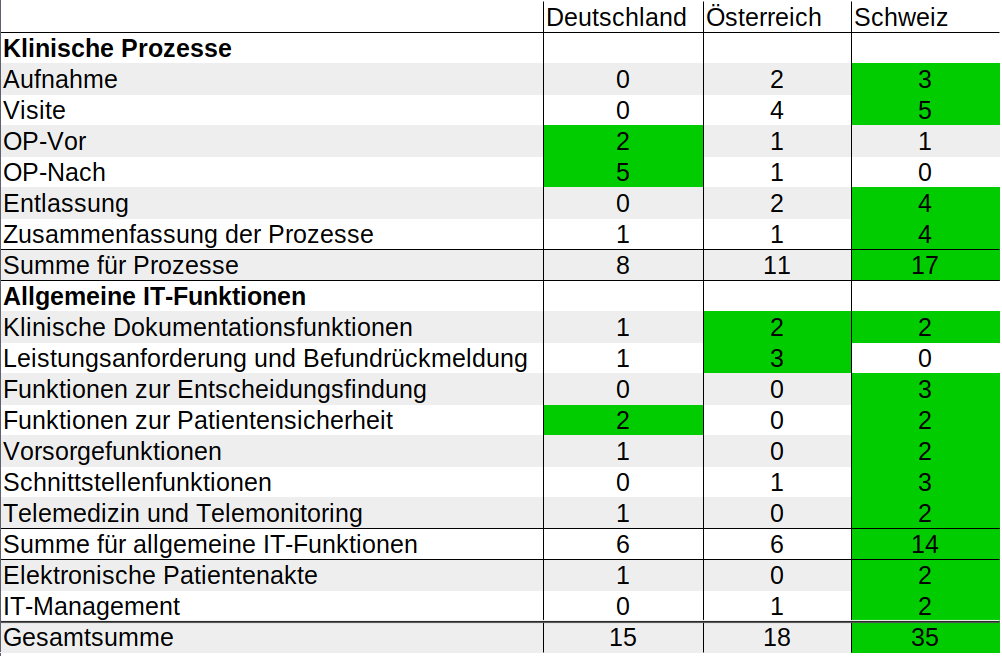
\includegraphics[width=0.7\textwidth]{Bilder/laendervergleich_ergebnisse.png}
	\caption{Ergebnisse des Ländervergleichs. Die Gewinner einer Kategorie sind grün markiert}
	\label{fig:laender_ergebnisse}
\end{figure}
Bei der gewählten Methodik ist zwar erkennbar welches Land die meisten Fragen gewonnen hat, aber nicht wie stark. Diese Ergebnisse geben also nur eine vergleichende und keine Qualitative Übersicht. Die Gegenüberstellung erfolgt nach der Struktur, die im IT-Report Gesundheitswesen 2020 vorgegeben ist. So werden zuerst die klinischen Prozesse betrachtet und anschließend verschiedene IT-Funktionstypen und das IT-Management. Eine Übersicht über die Ergebnisse befindet sich in Abbildung \ref{fig:laender_ergebnisse}.
\vspace{\parheadvspace}\\
\textbf{Klinische Prozesse}\\
In den Prozessen Aufnahme, Visite und Entlassung ist die Schweiz Vorreiter, während in den Unterstützungsprozessen des OP Deutschland führt. Es scheint, dass die externen Schnittstellen, Aufnahme und Entlassung, in Österreich und der Schweiz deutlich digitaler sind als in Deutschland. In der Visite zeigt sich vor allem eine höhere Verfügbarkeit von mobilen Geräten zum Zugriff auf Patientendaten und damit verbunden eine weitere Verbreitung von WLAN in Österreich und der Schweiz im Vergleich zu Deutschland. Daten im OP-Verlauf stehen in Deutschland jedoch deutlich häufiger in elektronischer Form bereit und die Informationsgüte ist höher, was sich am guten Abschneiden in der OP-Vorbereitung widerspiegelt. Bei der OP-Nachbereitung ergibt sich ein ähnliches Bild. Da OP-Daten in deutschen Krankenhäusern häufiger elektronisch verfügbar sind, können sie auch einfacher auf die Stationen übernommen werden. Die Zufriedenheit mit dem IT-Einsatz in den fünf Prozessen ist in der Schweiz am höchsten. Auch die Verfügbarkeit wesentlicher Patientendaten wird von schweizer Klinikern am besten eingeschätzt.
\vspace{\parheadvspace}\\
\textbf{Weitere IT-Funktionen}\\
Das Bild von der Schweiz als Vorreiter verdeutlicht sich bei der Betrachtung ausgewählter IT-Funktionen, die nicht klar einem klinischen Prozess zugeordnet werden. Lediglich bei \textit{Leistungsanforderung und Befundrückmeldung} schneidet Österreich besser ab. Während \textit{Funktionen zur Entscheidungsfindung} in Krankenhäusern aller drei Länder selten eingesetzt werden, sind diese in der Schweiz dennoch am verbreitetsten.
\vspace{\parheadvspace}\\
\textbf{Elektronische Patientenakte}\\
Während eine elektronische Patientenakte (ePA) in nur rund der Hälfte aller deutschen und österreicher Krankenhäuser zur Verfügung steht, haben über drei viertel aller Krankenhäuser in der deutschsprachigen Schweiz eine ePA implementiert. Wenn ein Krankenhaus eine ePA nutzt wird sie meistens im allen relevanten Einheiten genutzt.
\vspace{\parheadvspace}\\
\textbf{IT-Management}\\
Die Zufriedenheit mit dem IT-Support ist in Österreich und der Schweiz höher als in Deutschland. Zusätzlich ist die Integration der IT-Abteilung in der Schweiz am besten, wo es eine hohe Beteiligung des klinischen Personals an IT-Angelegenheiten gibt.

Im Allgemeinen ergibt sich bei Betrachtung der Daten des IT-Report Gesundheitswesen 2020 ein klares Bild: Die deutschsprachige Schweiz ist in Sachen Digitalisierung den andern Ländern vorraus, während Deutschland ehr Schlusslicht ist. Österreich befindet sich im Mittelfeld, ist aber deutlich näher an Deutschland als an der Schweiz. Das ist auch die Einschätzung in der Zusammenfassung des Report \parencite[29]{huebner2020}.

\subsection{Weitere Länder}
\begin{figure}[ht]
	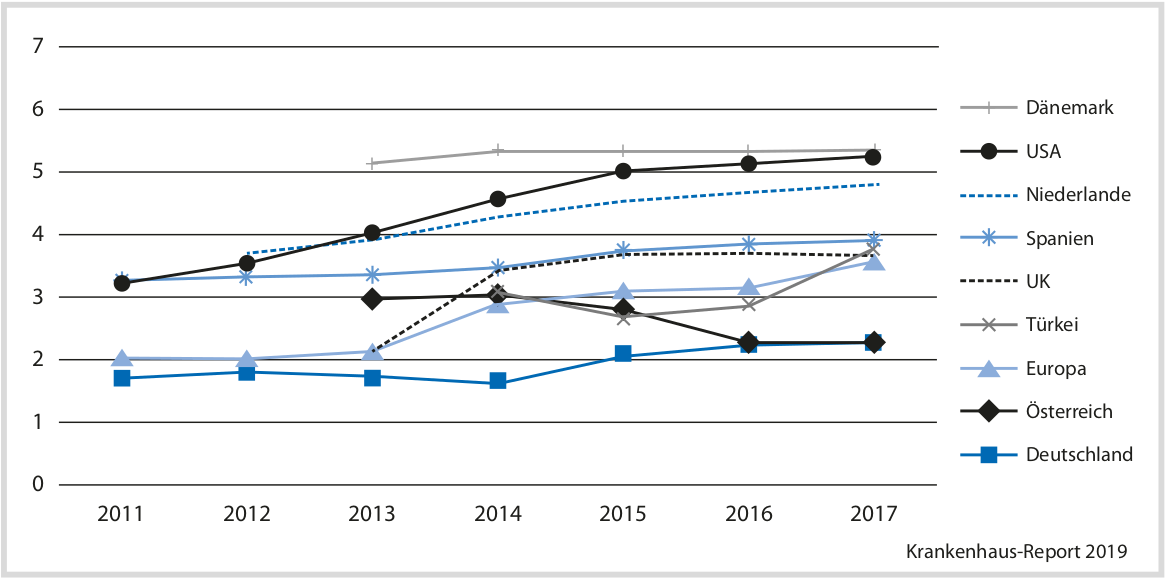
\includegraphics[width=0.95\textwidth]{Bilder/laendervergleich_EMRAM_Stephani_2019.png}
	\caption{Durchschnittliche EMRAM-Werte in ausgewählten Regionen seit 2011 \parencite{Stephani2019}}
	\label{fig:andere_laender}
\end{figure}
Für eine breitere Übersicht über den internationalen Stand der Digitalisierung an Krankenhäusern wird hier eine Übersicht des Schnitts der EMRAM Werte ausgewählter Länder von 2011 bis 2017 (siehe Abbildung \ref{fig:andere_laender}) aus \cite{Stephani2019} herangezogen. Eine Übersicht darüber wie diese Werte ermittelt werden befindet sich in Kapitel \ref{sec:EMRAM}. Es ist zu erkennen, dass Deutschland und Österreich mit einem Mittelwert von $2,3$ auf einem ähnlichen Niveau liegen, das deutlich unter dem europäischen Durchschnitt von $3,6$ liegt. Es gilt hier zu erwähnen, dass sich 167 deutsche Krankenhäuser über den Zeitraum zertifizieren lassen haben während es in Österreich nur 18 waren. Führende Länder in Europa sind die Niederlande ($n=36$) und Dänemark ($n=24$), mit einem jeweiligen Schnitt von $4,8$ und $5,4$. Die Türkei ($n=682$), das vereinigte Königreich($n=105$) und Spanien ($n=156$) liegen nahe am europäischen Mittel.


\section{Fazit}
% !TEX root = ../main.tex
Ähnlich wie in vielen anderen Sektoren liegt Deutschland im internationalen Vergleich mit Ländern ähnlicher Wirtschaftsstärke und Kultur beim Thema Digitalisierung auch im Krankenhausbereich hinten. Dies zeigt sich z.B. beim unterdurchschnittlichen Einsatz von mobilen Geräten wie Tablets und bedside Terminals.\\

Allgemein werden viele Informationen über Papier weitergeben, vor allem bei externen Schnittstellen, wie der Aufnahme und Entlassung. Dies liegt vor allem an der geringen elektronischen Vernetzung im gesamtheitlichen Gesundheitswesen. Es gibt die Hoffnung, dass sich diese Situation durch eine flächendeckende und einheitliche Implementierung der elektronischen Patientenakte verbessert.\\

In Krankenhäusern wird das Prinzip der IT-Governance selten angewandt und somit ist der Einsatz von IT nicht an vorderster Stelle, sondern Mittel zum Zweck.\\

Die aktuell hohe Auslastung der Krankenhäuser durch die Pandemie könnte sich auch negativ auf den Digitalisierungsfortschritt auswirken, da überlastetes Personal schwer für die Einführung neuer Systeme zu gewinnen ist. Dies ist durchaus berechtigt, da eine solche Änderung zwar langfristig Prozesse optimieren kann, aber immer auch eine Einarbeitungsphase hat. Nachdem diese unmittelbaren Probleme gelöst werden und sich die Situation entspannt, heißt es allerdings aus diesem Stresstest der Prozesse zu lernen und zu erarbeiten, wo der Einsatz von neuen Technologien sinnvoll die Arbeit der Kliniker ergänzt. Dabei wird es der neuen Generation von Ärzten und Pflegern, die vermehrt aus \textit{digital Natives} besteht, grundsätzlich leichter fallen neue Technik anzunehmen.\\

Die Einführung dieser Technologien wird zudem immer leichter, da Systeme ausgereifter sind und es mehr Beispiele für deren erfolgreicher Implementierung gibt. Dabei müssen deutsche Krankenhäuser auch nicht weit schauen, da es auch heute schon hochmoderne Krankenhäuser in Deutschland gibt, wie z.B. das Universitätsklinikum Hamburg-Eppendorf \parencite{Baehr2019}.

\newpage
\pagenumbering{Roman}
\setcounter{page}{3}
\listoftables
\newpage
\listoffigures
\newpage
\printbibliography
\addcontentsline{toc}{section}{Literaturverzeichnis}
\end{document}
